


In Figure \ref{fig:ml:classifier_errors} we show the error rates where \ref{fig:ml:classier_hist} is the histgram of securty values distributed over the label space. 
    
    \graphicspath{{resource/img/ch_ml/results/}}
    \begin{figure}
        \centering
        \begin{subfigure}[t]{1.5in}        
            \includegraphics[width=1.5in]{output_34_1.png}     
            \caption{}
        \end{subfigure}
        \begin{subfigure}[t]{1.5in}
            
            \includegraphics[width=1.5in]{output_37_1.png}  
            \caption{}
        \end{subfigure}
        \begin{subfigure}[t]{1.5in}
            \includegraphics[width=1.5in]{output_41_1.png}
            \caption{}
        \end{subfigure}
         \begin{subfigure}[t]{1.5in}
                
            \includegraphics[width=1.5in]{output_45_1.png}   
            \caption{}
        \end{subfigure}
    \medskip  % <-------------------------------  
        \begin{subfigure}[t]{1.5in}
            \centering
            % \caption{Prelec}
                \includegraphics[width=1.5in]{output_60_0.png}  
                \caption{}
        \end{subfigure}
    %            \caption{Prelec}%\label{fig:2b}
        \begin{subfigure}[t]{1.5in}
            \centering
                    % \caption{Prelec}
            \includegraphics[width=1.5in]{output_60_2.png} 
            \caption{}
        \end{subfigure}
        \begin{subfigure}[t]{1.5in}
            \centering
            % \caption{test}
            \includegraphics[width=1.5in]{output_60_4.png}
            \caption{}
        \end{subfigure}
            \begin{subfigure}[t]{1.5in}
            \centering
            % \caption{test}
            \includegraphics[width=1.5in]{output_60_6.png}
            \caption{}
        \end{subfigure}
        
            
    \medskip  % <-------------------------------  
            
           \begin{subfigure}[t]{1.5in}
            \centering
            % \caption{Prelec}
                \includegraphics[width=1.5in]{output_60_8.png}  
                \caption{}
        \end{subfigure}
    %            \caption{Prelec}%\label{fig:2b}
        \begin{subfigure}[t]{1.5in}
            \centering
                    % \caption{Prelec}
            \includegraphics[width=1.5in]{output_60_10.png} 
            \caption{}
        \end{subfigure}
        \begin{subfigure}[t]{1.5in}
            \centering
            % \caption{test}
            \includegraphics[width=1.5in]{output_60_12.png}
            \caption{}
        \end{subfigure}
            \begin{subfigure}[t]{1.5in}
            \centering
            % \caption{test}
            \includegraphics[width=1.5in]{output_61_1.png}
            \caption{}\label{fig:ml:classier_hist} 
        \end{subfigure}
        
        \medskip  % <-------------------------------  
            
           \begin{subfigure}[t]{1.5in}
            \centering
            % \caption{Prelec}
                \includegraphics[width=1.5in]{output_66_1.png}  
                \caption{}
        \end{subfigure}
    %            \caption{Prelec}%\label{fig:2b}
        \begin{subfigure}[t]{1.5in}
            \centering
                    % \caption{Prelec}
            \includegraphics[width=1.5in]{output_66_3.png} 
            \caption{}
        \end{subfigure}
        \begin{subfigure}[t]{1.5in}
            \centering
            % \caption{test}
            \includegraphics[width=1.5in]{output_69_1.png}
            \caption{}
        \end{subfigure}
            \begin{subfigure}[t]{1.5in}
            \centering
            % \caption{test}
            \includegraphics[width=1.5in]{output_71_1.png}
            \caption{}   
        \end{subfigure}
        
        \medskip  % <-------------------------------  
            
    %       \begin{subfigure}[t]{1.5in}
    %         \centering
    %         % \caption{Prelec}
    %             \includegraphics[width=1.5in]{output_73_1.png}  
    %             \caption{}
    %     \end{subfigure}
    % %            \caption{Prelec}%\label{fig:2b}
    %     \begin{subfigure}[t]{1.5in}
    %         \centering
    %                 % \caption{Prelec}
    %         \includegraphics[width=1.5in]{output_83_1.png} 
    %         \caption{}
    %     \end{subfigure}
    %     \begin{subfigure}[t]{1.5in}
    %         \centering
    %         % \caption{test}
    %         \includegraphics[width=1.5in]{output_85_1.png}
    %         \caption{}
    %     \end{subfigure}
    %         \begin{subfigure}[t]{1.5in}
    %         \centering
    %         % \caption{test}
    %         \includegraphics[width=1.5in]{output_97_0.png}
    %         \caption{}   
    %     \end{subfigure}
        \centering
        \caption{Classifier Error Plots (Predicted vs Actual) for the system's calculated security}\label{fig:ml:classifier_errors} 
    \end{figure}


% \begin{figure}
% \begin{tabular}{cccc}
% \subfloat[caption]{\includegraphics[width = 1.5in]{resource/img/ch_ml/results/output_34_1.png}} &
% \subfloat[caption]{\includegraphics[width = 1.5in]{resource/img/ch_ml/results/output_37_1.png}} &
% \subfloat[caption]{\includegraphics[width = 1.5in]{resource/img/ch_ml/results/output_41_1.png}} &
% \subfloat[caption]{\includegraphics[width = 1.5in]{resource/img/ch_ml/results/output_45_1.png}}\\
% \subfloat[caption]{\includegraphics[width = 1.5in]{resource/img/ch_ml/results/output_60_0.png}} &
% \subfloat[caption]{\includegraphics[width = 1.5in]{resource/img/ch_ml/results/output_60_2.png}} &
% \subfloat[caption]{\includegraphics[width = 1.5in]{resource/img/ch_ml/results/output_60_4.png}} &
% \subfloat[caption]{\includegraphics[width = 1.5in]{resource/img/ch_ml/results/output_60_6.png}}\\
% \subfloat[caption]{\includegraphics[width = 1.5in]{resource/img/ch_ml/results/output_60_8.png}} &
% \subfloat[caption]{\includegraphics[width = 1.5in]{resource/img/ch_ml/results/output_60_10.png}} &
% \subfloat[caption]{\includegraphics[width = 1.5in]{resource/img/ch_ml/results/output_60_12.png}} &
% \subfloat[caption]{\includegraphics[width = 1.5in]{resource/img/ch_ml/results/output_61_1.png}}\\
%  \subfloat[caption]{\includegraphics[width = 1.5in]{resource/img/ch_ml/results/output_66_1.png}} &
% \subfloat[caption]{\includegraphics[width = 1.5in]{resource/img/ch_ml/results/output_66_3.png}} &
% \subfloat[caption]{\includegraphics[width = 1.5in]{resource/img/ch_ml/results/output_69_1.png}} &
% \subfloat[caption]{\includegraphics[width = 1.5in]{resource/img/ch_ml/results/output_71_1.png}}\\
% \subfloat[caption]{\includegraphics[width = 1.5in]{resource/img/ch_ml/results/output_73_1.png}} &
% \subfloat[caption]{\includegraphics[width = 1.5in]{resource/img/ch_ml/results/output_83_1.png}} &
% \subfloat[caption]{\includegraphics[width = 1.5in]{resource/img/ch_ml/results/output_85_1.png}} &
% \subfloat[caption]{\includegraphics[width = 1.5in]{resource/img/ch_ml/results/output_97_0.png}}\\
% \subfloat[caption]{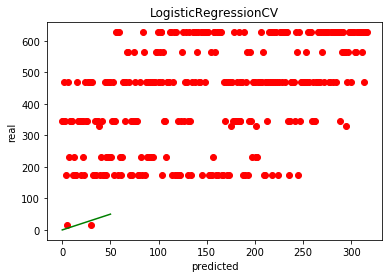
\includegraphics[width = 1.5in]{resource/img/ch_ml/results/output_112_1.png}} &
% \subfloat[caption]{\includegraphics[width = 1.5in]{resource/img/ch_ml/results/output_85_1.png}}
% \end{tabular}
% \caption{4 x 4}
% \end{figure}

% noderank hist: resource/img/ch_ml/results/output_61_1.png
% uniform hist: resource/img/ch_ml/results/output_63_2.png
% his grid: resource/img/ch_ml/results/output_51_0.png


% \begin{figure}%
%     \centering
%     \subfloat[label 1]{{\includegraphics[width=5cm]{img1} }}%
%     \qquad
%     \subfloat[label 2]{{\includegraphics[width=.5\linewidth]{resource/img/ch_ml/results/output_97_0.png} }}%
%     \caption{2 Figures side by side}%
%     \label{fig:example}%
% \end{figure}
